\documentclass[12pt]{article}
\usepackage[pdftex]{graphicx}
\usepackage{multicol}
\usepackage{html,makeidx}
\title{Generating and applying triangulations to Delaunay surfaces and combinatorial Ricci flows}
\pagestyle{plain}
\author{Alex Henniges \\ Thomas Williams \\ Mitch Wilson \\ \\ University of Arizona Undergraduate Research Program\\
Supervisor: Dr. David Glickenstein\\
}

\begin{document}

\maketitle
\thispagestyle{empty}
\newpage
\renewcommand\contentsname{Table of Contents}
\tableofcontents

\newpage
\section{Introduction}

The purpose of this paper is to explore and entend upon the use of triangulaitions in Delaunay surfaces and combinatorial Ricci flow. These concepts will be addressed under an analytical structure by designing a system to represent the triangulations and provide meaningful data. A large collection of data has not yet been compiled on these concepts and our goal is for such data to solidify as well produce theories in this fairly unexplored area of mathematics. The program used for this purpose will be written in C++.\newline

\noindent This paper will begin in $\S\ref{Triangulationschap}$ with an introduction to triangulations and any related definitions. Also, it will explain how our program is structured to meet its function. We will then present our research on Delaunay surfaces. That will be followed by an explanation of combinatorial Ricci flow along with the results from our initial experiments. In $\S\ref{HypSphere}$ we continue the exploration of Ricci flow under different geometries. Lastly, we will provide areas of future work on this subject.

\section{Triangulations}
\label{Triangulationschap}

Suppose you are asked to construct the surface of a sphere with as few pieces as possible. You could make a number of possible shapes, such as a cube or a soccer ball. While both of these shapes are discrete in nature, they can be used to approximate a round, continuous sphere. The most basic Euclidean approximation of the surface of a sphere is the boundary of a tetrahedron. Using only four vertices, six edges, and four faces, the tetrahedron is able to give us a surface that represents the surface of a sphere. Naturally, if we add more vertices, we are able to better illustrate our shapes through greater refinement. Similarly, in modern video games and Hollywood movies, various shapes are generated using polygons of many different sizes that mold to form a graphically rendered object. For these and all shapes, we will focus on building them solely out of triangles. Since any regular polygon can be broken up into triangles, we can essentially represent any surface using this method. \newline

\begin{figure}
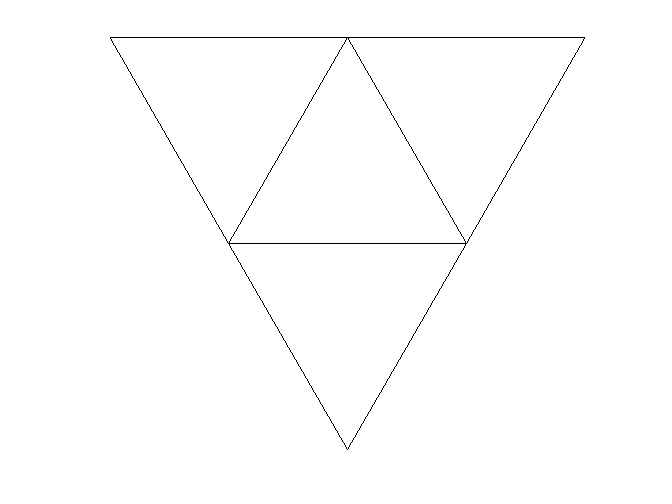
\includegraphics[scale = 0.5]{Pictures/flattetrahedron.png}
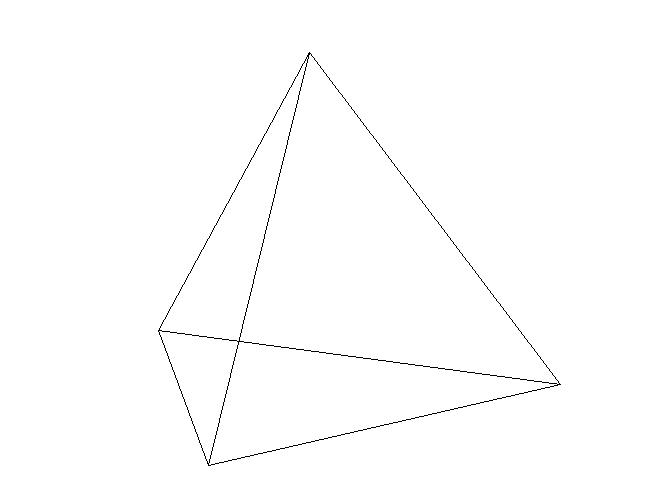
\includegraphics[scale = 0.3]{Pictures/tetrahedron.jpg}
\caption{An example of a triangulation. In this case, the triangle, a 2-simplex, can be folded up into the boundary of a tetrahedron, a 3-simplex.}
\end{figure}

\subsection{Basics and Definitions}

\noindent For an \textit{n}-dimensional space, this triangulation, written $\tau = \{\tau_0, \tau_1, ... , \tau_n\}$ consists of lists of simplices $\sigma^k$, where the super-script denotes the dimension of the simplex and $\tau_k$ is the list of all \textit{k}-dimensional simplices $\sigma^k = \{i_0, ... , i_k\}$ \cite{Dave}. We shall refer to 0-dimensional simplices as vertices, 1-dimensional simplices as edges, 2-dimensional simplices as triangles or faces, and 3-dimensional simplices as tetrahedra. For this project, we will only need to discuss triangulations of 2-dimensional spaces, or surfaces.\newline

\noindent In order to describe our surfaces we must make a definition for each individual simplex. For our data structure, we decided on creating a list of references for each simplex to give it definition within the triangulation. These lists of references for each simplex are refences to other simplices in the triangulation with the property of being local. We define the term ``local'' slightly different for each simplex. To begin with, we say that an edge is defined by two vertices and a face is defined by three vertices and three edges. Then, we can say that a vertex is local to any edge that it is in the definition of and any face that it is in the definition of, as well as any vertex that it shares an edge in common with. We say that a vertex has a \textit{degree} equal to the number of its local edge. An edge is local to any vertex that it is defined by and any face that it is in the definition of, as well as any edge that it shares a vertex in common with. A face is local to any vertex it is defined by, any edge that it is defined by, and any face that it shares an edge in common with. These are the definitions for locality of simplices that we decided upon, creating three different lists for each simplex. \newline

\noindent As well as lists of references to other simplices, each simplex also has other information needed to form a triangulation. While we say that these lists of references define the topology of a given triangulation, we must provide dimensions in order to define its geometry. Namely, each edge $\{i, j\}$ is given a length $l_{ij}$ and each vertex $i$ is given what we call a \textit{weight}, denoted by $r_i$. We think of the weight of a given vertex to be the radius of a circle centered at that vertex. We are then able to state that for any $\textit{n}$-dimensional simplex, there exists an $(n-1)$-dimensional sphere that is orthogonal to each of the spheres centered at the vertices which define that particular simplex\cite{Dave}. We use this particular sphere, and its center, to define the center of the given simplex. For our project, this means that a triangle $\{i, j, k\}$ has a center defined by the center of the circle which lies orthogonally to all of the circles at each vertex, also known as the orthocircle. Additionally, each edge also has a center defined by the weights and the length of the edge. \newline

\noindent Based on these centers, we are able to define the \textit{local lengths} of an edge, as well as the \textit{dual} of a given simplex, a concept that will become more important later on. For an edge $\{i, j\}$, it is true that 

$$l_{ij} = d_{ij} + d_{ji},$$

\noindent where $d_{ij}$ is the local length of edge $\{i, j\}$ from vertex $i$, or the length from vertex $i$ to C($\{i, j\}$), the center of $\{i, j\}$. If we examine the edge lengths of a given triangle, it can be concluded that 

\begin{equation}
d_{ij} = \frac{l_{ij}^2 + r_i^2 - r_j^2}{2l_{ij}}
\label{eq2}
\end{equation}

\noindent It also holds that 

\begin{equation}
\label{eq1}
d_{ij}^2 + d_{jk}^2 + d_{ki}^2 = d_{ji}^2 + d_{kj}^2 + d_{ik}^2
\end{equation}

\noindent for any face $\{i, j, k\}$. Based on this condition, we are guaranteed that for every face $\{i, j, k\}$, the perpendiculars from each edge center meet at a single point, which is the center of the face $C(\{i, j, k\})$ as defined above\cite{Dave}.\newline

\noindent There are two notable examples of choices of weights and their corresponding face centers. The first is when all of the weights are zero. In this case, a triangle center $C(\{i, j, k\})$ is the center of the circumcircle of $\{i, j, k\}$. The second is when the weights are equal to the local lengths for \textit{i}, or for all vertices \textit{j} and \textit{k} that are local to \textit{i}, we have $d_{ij} = d_{ik}$. This case is known as a \textit{circle packing} and will be used in the material discussed in $\oint\ref{RBk}$. In this case, a triangle center $C(\{i, j, k\})$ is the center of the incircle of $\{i, j, k\}$.

\noindent We will now make definitions for duals of our simplices. First, the dual of a face is simply its center $C(\{i, j, k\})$ as defined above. Now we will define a dual for a given edge. Let us refer to any edge, along with the faces of which it forms an intersection, as a \textit{hinge}. We are able to embed any hinge in the plane. Because of (\ref{eq1}), we know that on any hinge in the plane, the center of an edge along with the centers of its two local faces are colinear. The line connecting these three points is the dual for the given edge. We can determine the length of this dual if we can determine the length of the line segment connecting the center of an edge to the center of one of its local faces. On triangle $\{i, j, k\}$, we can write the distance between $C(\{i, j\})$ and $C(\{i, j, k\})$ as 

\begin{equation}
\label{eq3}
d[C(\{i, j\}), C(\{i, j, k\})] = \frac{d_{ik} - d_{ij}\cos(\theta_i)}{\sin(\theta_i)}
\end{equation}

\noindent where $\theta_i$ is the angle at \textit{i} on face $\{i, j, k\}$. In the case that $C(\{i, j, k\})$ lies outside of $\{i, j, k\}$, then this distance has a negative value. Otherwise, the distance is positive\cite{Dave}. Naturally, the dual of a given edge has a distance that is obained by adding the distances from the center of the edge to the centers of each face it is local to. The dual of a given vertex \textit{i} is the area enclosed by the duals of every edge local to \textit{i}. The duals of edges will be talked about again in \ref{DT}.\newline

\subsection{Bistellar moves}

\noindent On a given triangulation, we are able to perform different modifcations, which we will refer to as \textit{bistellar moves} or \textit{flips}. The are three possible bistellar moves that can be performed on a 2-dimensional triangulation: a 1-3 move, a 2-2 move, and a 3-1 move. One way to understand these moves, and where the term \textit{flip} comes from, is to imagine holding in your hand a tetrahedron. You can look at this tetrahedron three different way, at a face, at an edge, or at a vertex. If you were to ``flip over'' this object, you would see

\subsection{Programming Structure}

\noindent When creating the program, the data structure design was critical. The design not only helps dictate the direction of the project over the course of its lifespan, but the decisions affect the speed and efficiency of all added functionality. It was agreed that the system would have to hold the different simplices and that they would be referencing each other. This part of the program would need to be structured in a way that makes it quick and easy to move from one simplex to another. As seen in Figure \ref{triUML}, all simplices are assumed to have lists of references to other simplices, what we call local simplices, broken down by dimension. For the two-dimensional case, each simplex has lists of local vertices, local edges, and local faces.\newline

\noindent The lists are vectors of integers. The vector, provided in the C++ library, was chosen so that the list can dynamically change in size. The integers are a decision based on both speed and size. Instead of, for example, a vertex having a list of actual edges ($\overline{AB}, \overline{CF},$ etc.) or pointers to edges, the vertex has a list of integers representing the edges. The actual edges are then obtained through the $Triangulation$ class, which holds maps from integers to simplices. The $Triangulation$ class is made up of static functions and maps and is designed so only one triangulation exists at any time. Because the maps are static, they can be accessed at any time from anywhere in the code without the need to pass pointers through function calls. \newline


\section{Delaunay triangulations}
\label{DT}
\begin{itemize}
\item Definition of Delaunay triangulation
\item Plane generation algorithm with necessary equations
\item Math, flips, duals, negative triangles, equations, oh my!
\item Verifications, duals
\end{itemize}


\subsection{Definitions}
\noindent One special type of triangulation is known as a \textit{Delaunay Triangulation}, which we define as a set of faces on a plane such that the orthocircle defined by the three vertices of any given face do not enclose any other vertices. See Fig.~\ref{genTri} for an example with only a few faces. There are two main Delaunay cases, weighted and non-weighted. In non-weighted, the orthocircle about the face is made to intersect all three vertices, and thus is the circumcircle. In a weighted Delaunay case, the orthocircle surrounding a face remains orthogonal to the radius of the circle of each vertex. Delaunay triangulations have particular interest in the fields of Computer Science and Physics.\newline


\begin{figure}
\centering
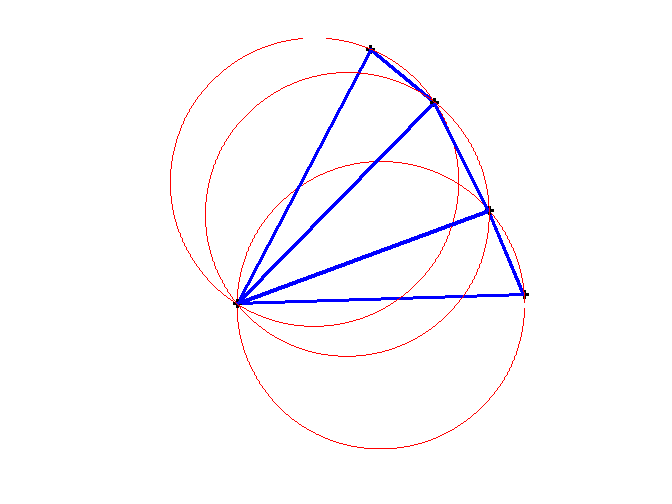
\includegraphics[scale = 0.6]{Pictures/genTri4.png}
\caption{A simple example of a Delaunay triangulation. The circumcircles are drawn along with the edges to show their compatability. This is a non-weighted case.}
\label{genTri}
\end{figure}

\noindent We can produce a non-weighted Delaunay triangulation using mathematical software like MATLAB. However, less is known about weighted triangulations in general. For this project, we aim to develop an algorithm that can create a valid triangulation, add weights to vertices, and manipulate the faces to produce a Delaunay triangulation.\newline

\noindent An important aspect to properly explore these triangulations is in their generation. We developed a program $generateTriangulation$ which can generate a determined number of faces with a random configuration. To truly test our algorithms and to provide convincing results would require an unbiased way of constructing the triangulations. There are several properties to triangulations that we wish to be randomized, and they include the lengths of each edge, the degree of each vertex, and the weight at each vertex. It is unclear if there is a way to provide a truly random generation of triangulations or even if such a system would be desirable, but we feel that the algorithm we chose adequately meets our goals.\newline

\noindent Our random triangulation generator begins with one triangle with edge lengths between zero and ten. This was chosen arbitrarily as all future weights will be based off of these. Triangles are then created from each edge along the border. When the creation of an edge would result in a vertex's angles summing to greater than $2\pi$, we instead close off the vertex by connecting its two outer edges. Once the desired number of faces have been created, the algorithm ends. Section [] in the appendix shows several results of this algorithm.\newline

\begin{figure}
\centering
\includegraphics[scale = 0.45]{Pictures/gentri.png}
\includegraphics[scale = 0.45]{Pictures/gentri6.png}
\caption{Two examples of triangulations using our $generateTriangulation$ program, an early version (left) and a modern version (right).}
\end{figure}

\noindent We can generate weights at random by restricting their maximum size with respect to the shortest edge length in the triangulation, so as not to make weights too large. We can also assign weights to individual vertices such that others remain unweighted. \newline

\noindent In order for a triangulation that we have created to be Delaunay, we must be able to guarantee that all orthocircles behave as they should. However, in our gereration, we can create triangles in which the largest side length is barely smaller than the sum of the other two sides, or ``skinny triangles.'' We find that the orthocircles related to these triangles have a large tendency to make the triangulation not Delaunay as they like to contain other vertices. To remedy this issue, we aim to perform manipulations known as \textit{flips}. Also known as \textit{bistellar moves}, these slight alterations aim to make the triangulation Delaunay. \newline

\noindent In particular, we will focus on one flip known as the 2-2 flip. In this flip, we take a pair of adjacent faces and readjust the edge that they share to connect the opposite pair of vertices, as shown in figure~\ref{fig:flip}. This move creates no new simplices and removes no existing vertices. The code for the 2-2 flip is located in $\oint\ref{calcFlowCode}$. We will discuss other flips in []. \newline

\noindent We feel that if a triangulation if not Delaunay, we can perform a series of 2-2 flips on various surfaces until it results in a Delauany configuration. We do not change the vertices in any fashion or the number of triangles, only how they are connected to each other. \newline

\begin{figure}
\centering
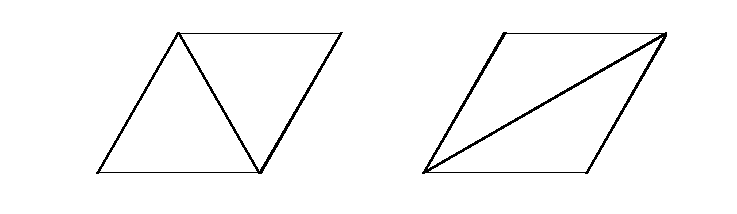
\includegraphics[scale = 0.8]{Pictures/Flip.png}
\caption{An example of a 2-2 flip.}
\label{fig:flip}
\end{figure}

\noindent One issue we noted was that certain flips would change our notion of triangles. Flips sometimes produced triangles where they did not exist before. We call these anti-triangles, or \textit{negative triangles}. See Figure~\ref{AntiTri}. We can check for cases when this may happen and adapt our flipping process as needed. \newline

\noindent We know that anti-triangles are related to the dual lengths associated with the faces (See $\oint$2.3). If the center of a triangle is outisde the triangle itself, we say that the dual has a negative length. Similarly, we say that a negative triangle has a negative area in order to conserve area, as can also be seen in Fig.~\ref{AntiTri}. \newline

\begin{figure}
\centering
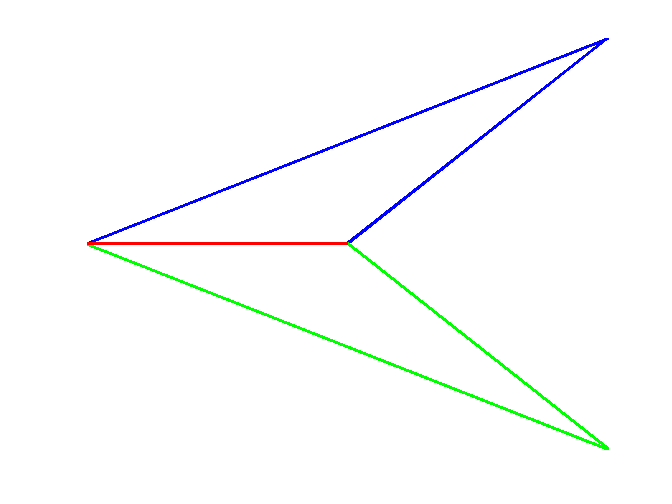
\includegraphics[scale = 0.4]{Pictures/antitri1.png}
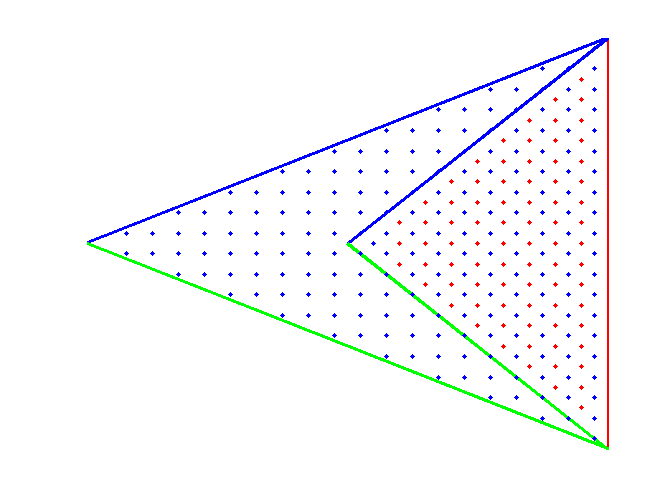
\includegraphics[scale = 0.4]{Pictures/antitri2.png}
\caption{If flips are performed on nonconvex triangles, we create an anti-triangle, shaded here in red, and a larger regular triangle, shaded in blue.}
\label{AntiTri}
\end{figure}

\noindent We created a program called $weightedFlipAlgorithm$ that scans each face to see if it was Delaunay, and if not, we would perform a flip with an adjacent face. We would repeat the process until (hopefully) each face was Delaunay, and thus the whole triangulation was now Delaunay. Unfortunately, the process did not always end. \newline

\noindent To get a better grasp of the evolution of the flips, we made a MATLAB program named $delaunayPlot$ that would draw a triangulation so we could visually ensure that our triangulations were being built correctly and also if and where flips were being performed, as well as tracking negative triangles. We use MATLAB as it is able to read data from files, like in C++, as well as generate pictures relatively easily. We adapted this code to then make $multiDelaunayPlot$, which regraphs the triangulation after a flip is performed. \newline

\noindent Often times, we did find that triangulations were able to become Delaunay after a series of flips. As we added more faces, and increased weights by scalars, we noted that it was more likely for the algorithm to have issues. In watching our $multiDelaunayPlot$ results, we found that certain edges would loop in a series of flips such that performing one flip would require the adjacent edge to need flipping. Occasionally, one edge would get stuck flipping back and forth between two faces. We also noted that final triangulations did permit the existence of negative triangles. Often they were found on the edge boundary and of little concern. We were able to check our results by drawing the dual edges on top of all the faces using equations from []. If all vertices had zero weight, then the duals are simply the perpendicular bisectors of each edge. See Figure~\ref{Duals}. \newline

\begin{figure}
\centering
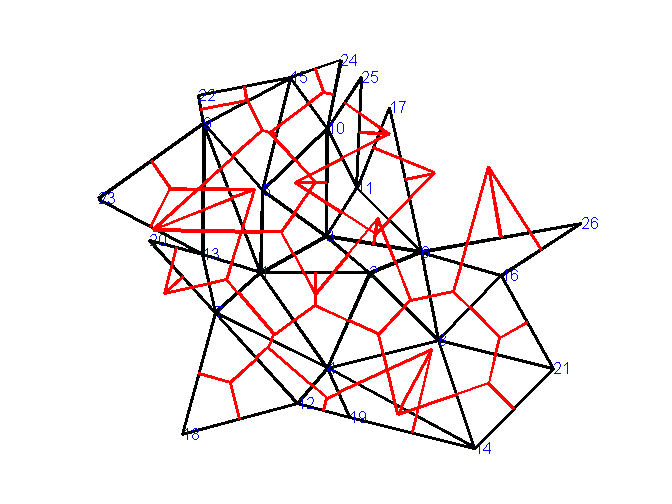
\includegraphics[scale = .45]{Pictures/nonwduals.png}
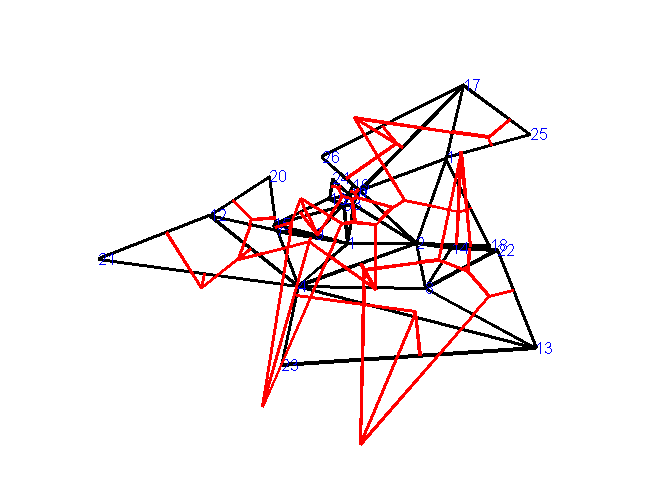
\includegraphics[scale = .45]{Pictures/Wduals.png}
\caption{A non-weighted (left) and weighted (right) triangulation with dual lengths added.}
\label{Duals}
\end{figure}

\noindent We also observed a couple of interesting things from a statistical point of view. We found that, after flips were performed, the average length of all edges tended to decrease by a small amount. This would lead to suggest that vertices try and form triangles with vertices close to itself, resulting in fewer skinny triangles. We also saw that the degrees of vertices tend to vary more after flips; more have a degree of 2, while others increase in degree. This indicates that the proximity of vertices to each other in its triangulation also has a great effect as well as the weights. See Figure~\ref{stats} for an example with a non-weighted case.\newline
\begin{table}
\begin{center}
\begin{tabular}{|rrr|rrr|}
 \hline
 &Scalar = 1.0      &            &            &  Scalar = 1.5           &          \\ \hline

   Faces & Avg. Flips & \% Finish &               Faces & Avg. Flips & \% Finish \\ \hline

        25 &        4.1 &        100 &                    25 &       13.5 &      83.33 \\

        50 &       11.2 &        100 &                     50 &       19.6 &      71.29 \\

       100 &       26.8 &        100 &                   100 &       41.7 &         40 \\ \hline

\end{tabular} 
\end{center}
\caption{An anlysis of number of flips required to obtain Delaunay triangulation for a given number of faces and scaled weights. Each test was performed on $weightedFlipAlgorithm$ until each test had ten successful runs. Each trial had unique weights.} 
\end{table} 

\begin{figure}
\centering
\includegraphics[scale = 0.6]{Pictures/Stats.png}
\caption{A statistical illustration of edge lengths and vertex degrees before and after flips are performed.}
\label{stats}
\end{figure}

\noindent So to conclude, yeah, flips are awesome. 

\section{Combinatorial Ricci flow}
\label{RBk}

Introduced by Richard Hamilton in 1982, Ricci flow, named in honor of Gregorio Ricci-Curbastro \cite{RicciBkgd}, has since had a large influence in the world of geometry and topology. It is often described as a heat equation. Imagine a room where a fireplace sits in one corner and a window is open on the other side. The heat will diffuse through the room until the temperature is the same everywhere. With Ricci flow, the same occurs with the curvature. Under Ricci flow, a geometric object that is distorted and uneven will morph and change as necessary so that all curvatures are even.The biggest consequence of Ricci flow came when Grigori Perelman proved the Poincar\'{e} Conjecture in 2002. The Poincar\'{e} Conjecture, proposed in 1904, was particularly difficult to prove, and was given the honor of one of seven millennium puzzles by the Clay Mathematics Institute. It was Ricci flow that turned out to be the cornerstone for the proof. In addition, its relation to the heat equation may open new doors for work in fluid dynamics and even in the theory of general relativity \cite{RicciBkgd}. In 2002, Chow and Luo introduced the concept of combinatorial Ricci flow. They showed that this new concept, performed on a triangulation of a manifold, had many of the properties of the Ricci flow Hamilton had defined. That the subject is still very new makes this research project exciting. \newline

\subsection{Definitions and Equations}
We define a manifold to be a topological space where every neighborhood is locally Euclidean. This means that around any point in the space it appears similar to the sphere locally. What this means for our triangulated surfaces is that there are no borders. We also refer to this as a closed triangulation.\newline

\noindent When talking about closed, triangulated surfaces an important characteristic is known the Euler characteristic $\chi$, defined by the equation $\chi = V - E + F$, where \textit{V} is the number of vertices in the triangulation, \textit{E} is the number of edges, and \textit{F} is the number of faces. This characteristic is directly connected to another important property, the \textit{genus} of a surface. The genus of a surface is the toplogical property that is more loosely known as the number of ``holes'' in the surface. For instance, a sphere has a genus of 0 while a torus has a genus of 1, a two-holed torus has genus 2, etc. The relationship between the two values is given by $\chi = 2 - 2g$, where \textit{g} is the genus of the surface.\newline 

\noindent Once we have a triangulation and it is circle packed, vertices can be too large or too small, and the resulting geometry can be somewhat intractable. We would like to have a way to determine the evolution of each shape to its final form, which may be more uniform. We introduce combinatorial Ricci flow to the sytem. On a discrete surface, this equation allows the weights to change over time \cite{chowluo}. We present the equation to the reader, which can be written as

  \begin{equation}
  \label{Riccif}
  \frac{dr_i}{{dt}} = -K_ir_i
  \end{equation}
  
\noindent where $K_i$ is a characteristic called the $curvature$ of a vertex, and $r_i$ is the $radius$ or $weight$ of the vertex $i$. We use the words ``radius'' and ``weight'' interchangeably, denoting the length of the radius that surrounds a vertex $i$ in circle-packing. The value of $K_i$ changes with time. Its value is found by determining the angles of all triangles containing vertex $i$. Using side lengths we can determine the angle using the law of cosines. For a triangle with lengths $a, b,\mbox{ and }c,$ the angle opposite side $c$ is
  
  $$
  \angle C = \arccos(\frac{a^2 + b^2 - c^2}{2ab})
  $$
  
\noindent with similar formulas for the other angles. We take the sum of all angles associated with a vertex $i$ and define the curvature $K_i$ as

\begin{equation}
K_i = 2\pi - \sum{\angle i}.
\end{equation}
  
\noindent Since we are performing multiple non-linear differential equations as variables depend on the weights which change over time, we can probably not solve them explicitly.\newline
   
\noindent A potential issue we noted is that, based on the equation, is it possible that the radii could continually decrease. Take, for example, a simple tetrahedron with all sides of equal length. We find that the curvature of each vertex always equals $\pi$. Thus in solving the differential equation computationally we would decrease each vertex by the same amount, but the curvature of each vertex would still remain $\pi$ because the curvature is not affected by uniform scaling. The radii would continue to decrease until they approach zero length. We have to address that issue since computers don't like working with numbers near zero, as in the denominator of the arccosine function. Numerical instability may occur. To avoid this issue, let us resize the length of each radius by a scalar, $\alpha$. We denote each scaled length by $\tilde{r_i}$ and equate as
 
$$ \tilde{r_i} = \alpha r_i. $$ 
 
\noindent Each $\tilde{r_i}$ would have its own $\tilde{K_i}$, but since we are scaling all sides by the same factor, this does not effect the curvature of the surface, so $\tilde{K_i} = K_i$. Thus in plugging $\tilde{r_i}$ in to the differential equation we get
 
 \begin{eqnarray}
 \label{ref1}
 \frac{d\tilde{r_i}}{dt} &=& \frac{d(\alpha r_i)}{dt} = \alpha \frac{dr_i}{dt} + r_i\frac{d\alpha}{dt}\nonumber\\
 &=& -\alpha K_ir_i + \frac{\tilde{r_i}}{\alpha}\frac{d\alpha}{dt} \nonumber \\
 &=& -\tilde{K_i}\tilde{r_i} + \frac{\tilde{r_i}}{\alpha}\frac{d\alpha}{dt}.
 \end{eqnarray}
 
\noindent We also note that $\displaystyle \frac{1}{\alpha} \frac{d\alpha}{dt} = \frac{d(\log \alpha)}{dt}$ using a basic chain rule. In order to find an appropriate value for $\alpha$ we decided to use the following criterium:
 
\begin{equation}
\label{eqprod}
f(\tilde{r_1},\tilde{r_2},\ldots,\tilde{r_n}) = \prod{\tilde{r_i}} = \prod{\alpha r_i} = C\mbox{, a constant.}
\end{equation}

\noindent We will call this value the \textit{product area} of the surface. This area prevents all radii from decreasing to zero at the same time. By taking the derivative of Eq.~($\ref{eqprod}$) with respect to time we find that 
 
\begin{equation}
\label{proof1}
\frac{d(\mbox{log}~\alpha)}{dt} = \frac{\mbox{sum of all curvatures}}{\mbox{number of vertices}} = \overline{K}, \mbox{average curvature.}
\end{equation}

\noindent In this paper, we may refer to the sum of all curvatures as the \textit{total curvature}. We can also show that $\overline{K}$ is a constant and depends on the number of vertices and the Euler characteristic. We know that the sum of angles from each vertex is $360^\circ,$ or $2\pi$. However, we also know that the sum of angles on each face is $\pi$, thus we determine that 

$$\sum{K_i} = 2\pi V - \pi F = 2\pi(V - \frac{F}{2})$$

\noindent We can simplify this by noting trends in basic triangulations. As every face is made up of three edges, and each edge belongs to two faces, we can see that $3F = 2E, \mbox{or } E = \frac{3F}{2}$. Looking back at Table \ref{EuChar} we note this true for all polyhedra listed. Let us use this substitution and rewrite the above equation as

$$\sum{K_i} = 2\pi(V - \frac{F}{2}) = 2\pi(V - \frac{3F}{2} + F) = 2\pi(V - E + F) = 2\pi \chi.$$

\noindent Thus we find that $\overline{K}$ is just $\displaystyle\frac{\sum{K_i}}{|V|} = \frac{2\pi \chi}{|V|}$ where $|V|$ is the number of vertices. This is also noted in \cite{chowluo}. Plugging this information back into Eq.~($\ref{ref1}$) we determine that

\begin{equation}
\frac{d\tilde{r_i}}{dt} = -\tilde{K_i}\tilde{r_i} + \overline{K}\tilde{r_i} = (\overline{K} - \tilde{K_i})\tilde{r_i}
\end{equation}

\noindent However, since everything is now a function of $\tilde{r_i}$ and not $\alpha$, we can just as easily plug $r_i$ back in to the differential equation instead of $\tilde{r_i}$, so we end up with:

\begin{equation}
\label{Riccin}
\frac{dr_i}{dt} = (\overline{K} - K_i)r_i
\end{equation}

\noindent This is known as normalized Ricci flow, as discussed by Chow and Luo in their paper \cite{chowluo}. In the case of our basic tetrahedron from earlier, the radii would not change after each iteration as $\overline{K} = K_i = \pi$ and thus $\displaystyle\frac{dr_i}{dt} = 0$ for $i = \{1,2,3,4\}$. 

\subsection{Programming Ricci flow}
\noindent The function $calcFlow$ runs a combinatorial Ricci flow on a triangulation and records the data in a file. The algorithm for solving the ODE, provided by J-P Moreau, employs a Runge-Kutta method of order 4 \cite{JPM}. First, the file name for the data is provided. Then, a $dt$ is given by the user that represents the time step for the system. The next parameter is a pointer to an array of initial weights to use. This is followed by the number of steps to calculate and record. Lastly, a boolean is provided, where $true$ indicates that the normalized differential equation, (\ref{Riccin}), should be used. Otherwise, the standard equation (\ref{Riccif}) is employed. Each step, with every vertex's weight and curvature at that step, is printed to the file. An example is shown in Table~\ref{tab:ricciSteps}.\newline

\begin{table}
\begin{center}
\begin{minipage}{2.2in}
%\begin{multicols}{2}
\begin{tabular}{l|l|l}
\hline
Step 1   & Weight &  Curv\\
Vertex 1:& 6.000 & 0.7442\\
Vertex 2: &3.000 & -1.122\\
Vertex 3:& 3.000 & -1.373\\
Vertex 4:& 8.000 & 1.813\\
Vertex 5: &6.000 & 1.227\\
Vertex 6: &2.000 & -3.046\\
Vertex 7: &4.000 & -0.3045\\
Vertex 8: &8.000 & 1.989\\
Vertex 9: &5.000 & 0.07239\\ \hline
\end{tabular} 
\end{minipage}
\begin{minipage}{2.2in}
\begin{tabular}{l|l|l}
\hline
Step 50 &  Weight &  Curv\\
Vertex 1:& 4.557 & 0.008509\\
Vertex 2: &4.530 & -0.01185\\
Vertex 3: &4.534 & -0.009091\\
Vertex 4:& 4.563 & 0.01268\\
Vertex 5:& 4.550 & 0.002772\\
Vertex 6: &4.527 & -0.01455\\
Vertex 7: &4.541 & -0.003563\\
Vertex 8: &4.559 & 0.01018\\
Vertex 9: &4.553 & 0.004906\\ \hline
\end{tabular}
\end{minipage}
%\end{multicols}
\end{center}
\caption{Two steps of a Ricci flow}
\label{tab:ricciSteps}
\end{table}

\noindent After the initial design of $calcFlow$, tests were run to determine its speed. The time it took to run was directly proportional to the number of steps in the flow. However, it was also proportional to more than the square of the number of vertices of the triangulation. As a result, while a four-vertex triangulation can run a 1000 step flow in three seconds, it would take a twelve-vertex triangulation 43 seconds to run the same flow. After inspecting the speed of the non-adjusted flow in comparison, it became clear that the calculation of total curvature, which remains constant in two-dimensional manifold cases, was being calculated far too often. After being adjusted so that it is calculated just once per step, the speed of the flow is much faster so that a four-vertex system with 1000 steps takes just one second and twelve vertices is much improved with a time of only four seconds. The code for the $calcFlow$ function can be found in $\oint\ref{calcFlowCode}$.

\subsection{Initial testing and results}
We have some expectations for combinatorial Ricci flow over two-dimensional Euclidean surfaces. Cases like the boundary of the tetrahedron can be calculated by hand so it will be useful to test our results against these surfaces. For example, we expect that the tetrahedron under (\ref{Riccif}) will have all weights converge to zero. Whereas under (\ref{Riccin}) the weights are expected to converge to positive constants.\newline

\noindent There are other expected behaviors. We expect that the product of the initial weights will be equal to the product of the weights at any intermediate step of the flow, what we call the \textit{product area}. Also, it is predicted that the total curvature of a 2-manifold surface should remain a constant determined by its genus.\newline

\noindent For the program we expect to create a system that allows for easy access of information while also providing that information in a time efficient way. Our goal is to create a program that can be built upon later to provide further functionality and options without requiring widespread and time consuming changes to the code. While we certainly expect a number of bugs, we plan to develop methods to test and find any errors in our code. \newline

\noindent Initial checks for accuracy:
\begin{enumerate}
\item Boundary of tetrahedron will converge to equal weights.
\item Constant \textit{product area}.
\item Constant total curvature.
\end{enumerate}

\subsubsection{First tests}
\label{InitialResults}
The program for the Ricci flow was tested by beginning with the simplest cases, and then explored with as many different possibilities as we could conceive of to try to find anomalies. The first test was the boundary of the tetrahedron. In the standard equation, it is easily shown that all weights approach zero exponentially fast. In the normalized equation, and the equation that is used in the rest of the testing, the tetrahedron's weights approach a single positive number, the fourth root of the \textit{product area} of the tetrahedron, so that the area remains constant. In addition, all the curvatures converged to the same value, in this case $\pi$, so that the total curvature is $4\pi$. Results were similar for the other platonic solids.\newline

\noindent The next test was the torus with the standard nine-vertex triangulation. Again all the weights approached the same positive number to maintain constant area. As expected, the curvatures all went to zero while the total curvature remained zero throughout. Further simple tests included triangulations of larger genus, and in all cases the total curvature remained at a constant multiple of $\pi$ that was expected and the \textit{product area} was also constant. In addition, there does not appear to be any further effect from the initial weights other than determining the area of the triangulation. It is not clear from any of the tests we ran that having extremes amongst the initial weights causes a different end result.\newline

\noindent In each case all vertices converged to the same curvature. This was not always the situation for the weights, as in many triangulations there would be several final weights. It became clear that this would occur when vertices had different degrees. In fact, we guess that there is a formula relating the \textit{product area} of a weighted triangulation and the degree of a vertex to that vertex's final weight. In most of the examples we tried, when two vertices had the same degree, they had the same final weight, but this is not always the case. One such example is adding three vertices to one face of the tetrahedron. As seen in Table \ref{tab:weightTab}, vertices 4, 5, and 6 all have degree four. Yet vertex 5 has a greater final weight than the other two. The only explanation we could find with some merit is that the local vertices of 5 are different in degree from those of 4 and 6. That is, the degrees of the local vertices of 5 are never less than four, while vertices 4 and 6 each have a local vertex with degree 3. See Figure \ref{fig:t7vh} in the Appendix for an illustration of weights over time.\newline 


\begin{table}

\begin{minipage}[ht]{0.5\linewidth}

\begin{tabular}{|l|l|}
\hline
 Vertex: 1 &  Vertex: 5 \\
\hline
2 3 4 5 6 7  &   1 2 4 6  \\

1 2 3 7 10 13  &  7 8 9 12  \\

1 2 3 5 7 9  &   5 6 7 8  \\
\hline
 Vertex: 2 &  Vertex: 6 \\
\hline
1 3 4 5 6 7  &   1 2 5 7  \\

1 4 5 8 11 14  & 10 11 12 15  \\

1 2 4 6 8 10  &  7 8 9 10  \\
\hline
 Vertex: 3 &  Vertex: 7 \\
\hline
    1 2 4  &     1 2 6  \\

    2 5 6  &  13 14 15  \\

    2 3 4  &    1 9 10  \\
\hline
 Vertex: 4 &  Edge: 1    \\ 
\hline
  1 2 3 5  &   :         \\

  3 4 6 9  &   :         \\

  3 4 5 6  &            \\ 
\hline

\end{tabular}


\end{minipage}
\begin{minipage}[b]{0.5\linewidth}

\begin{tabular}{|l|}
\hline
Final weights for a random \\

initial weighted Triangulation \\
\hline
Vertex 1: 15.692 \\

Vertex 2: 15.692 \\

Vertex 3: 6.18421 \\

Vertex 4: 9.6524 \\

Vertex 5: 10.6409 \\

Vertex 6: 9.6524 \\

Vertex 7: 6.18421 \\
\hline
\end{tabular}
\end{minipage}
\caption{Adding three vertices to a Tetrahedron}
\label{tab:weightTab}
\end{table}


\subsubsection{Specific cases}

\noindent \textit{Example}: Adding a vertex to a one-holed torus. See figure~\ref{torusaddv}. \newline

\noindent By inserting a vertex within a triangulation for a torus, we are essentially creating a bump on the torus and then observe what happens as we run it through out $calcFlow$ program. We discovered that the new vertex shrinks in size to a weight much smaller than the other vertices, but to a positive constant. To counter this, the other vertices grow slightly to maintain Eq.~(\ref{eqprod}). The weight that the new vertex converges to turned out to be in proportion to the other weights by $3+2\sqrt{3}$, the exact proportion necessary to maintain equality amongst all other weights. An oddity here is that the three vertices local to this added vertex converged to the same weight as all the vertices not near the flip, despite a difference in degree.\newline

\begin{figure}[ht]
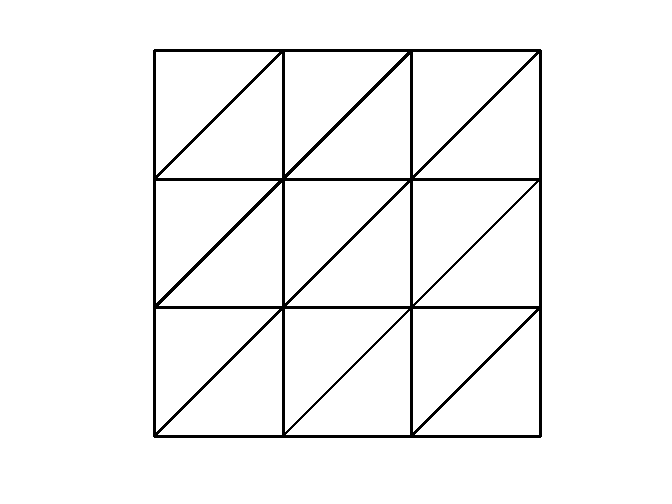
\includegraphics[scale = 0.5]{Pictures/torus22.png}
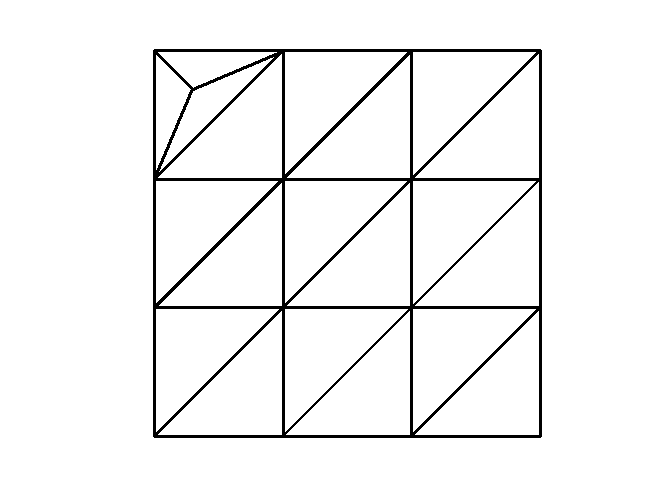
\includegraphics[scale = 0.5]{Pictures/torus2addvertex2.png}
\caption{A triangulation of the torus, and the addition of a new vertex. This is a 1-3 flip.}
\label{torusaddv}
\end{figure}

\noindent \textit{Example}: Adding a leaf to a two-holed torus.\newline

\noindent When we added a double triangle to the edge of a two-holed torus, we experienced for the first time what is known as a singularity. At the special vertex that was only of degree two, its weight continued to shrink and never converged. Eventually, enough steps of the Ricci flow were performed that the size of the weight became less than what the computer could differentiate from 0 and the program crashed with a division-by-zero error. Before the crash, the other vertices were increasing without convergence to counteract the decreasing weight. The reason is that all vertices wanted to attain the same curvature, in this case $-\frac{2}{5}\pi$. Yet the new vertex, with only two angles in its sum, can only obtain a curvature of 0 (each angle $\sim\pi$ radians). The result is that the weight shrinks in an attempt to attain angles greater than $\pi$, which is simply not possible. What is still not clear is whether or not the weight reaches 0 in finite time, or simply approaches 0. This is difficult to test with a computer only capable of approximating the weight, though we expect that it does so in finite time.\newline

\noindent \textit{Example}: Performing a 2-2 flip on a 12-vertex torus. \newline

\noindent One interesting observation we made was that flips can drastically change the behavior of some triangulations. For Example, in a 12-vertex torus, performing a flip on one edge affected created a double triangle. Similarly to the previous case, all curvatures are converging to 0, but the vertex with degree 2 simply cannot accomplish this. However, unlike the previous case, we suspect that the weight does not become 0 in finite time, but instead approaches 0.\newline

\noindent \textit{Example}: Triangulation of genus 4.\newline

\noindent While the previous two cases were quite interesting, there is some hesitation given that we were using double triangles and being less restrictive in what were allowable triangulations. But the theory behind why both situations reacted as they did left hope for a case that fit in a stricter setting. In the same sense that a two degree vertex could have a curvature no less than 0, a three degree vertex is bounded below by $-\pi$. It was observed that the vertices of a triangulation all converge to $\displaystyle\frac{2\pi\chi}{|V|}$ curvature. Now it was a matter of finding a triangulation with a large enough genus and few vertices. The first we found, provided by \cite{lutzmanifold}, was an 11 vertex triangulation with genus 4. To create a vertex with degree 3, we chose to add a new vertex to a face with a 1-3 flip. This made all curvatures try to converge to $-\pi$. We then expected that the new vertex would react as in the previous example. This was in fact the case, and it presents the question of whether or not there is a limit on the degree that can create such a singularity. The issue being that for higher genus, more vertices are required. Unfortunately, \cite{lutzmanifold} does not provide large enough triangulations for fourth degree vertices. A data plot of this similiar situation with a genus 6 triangulation is provided in $\S\ref{dataplots}$. \newline

\noindent \textit{Example}: Two tetrahedra connected at a vertex. See Figure \ref{fig:tt}\newline

\noindent It turns out $\chi = $ 7 Vertices - 12 Edges + 8 Faces = 3, which is not a case we had seen before. In previous cases $\chi$ was an even integer. Starting each vertex with equal weight, we obtained an unexpected result. The center weight becomes very large, and the others become smaller in comparison. We concluded that since the central vertex has a much higher degree, its weight becomes large, creating elongated tetrahedra on either side, in order to have the same curvature as all other vertices. One good thing we noted was that the total curvature equaled $6\pi = 2\pi\chi$. Technically, this example contradicts our notion of a manifold, but we felt it useful in validating our program procedure.  

\begin{figure}
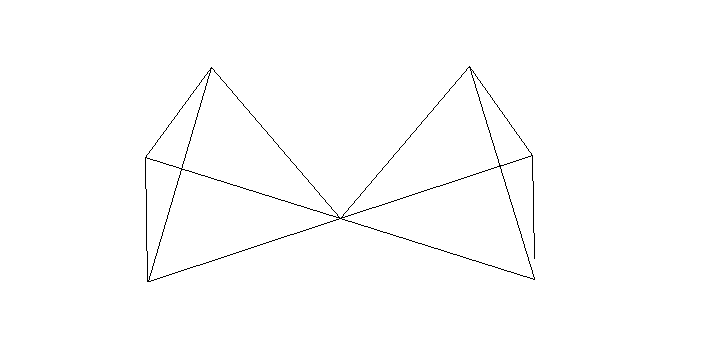
\includegraphics{Pictures/tetratouch.png}
\caption{Two tetrahedra conjoined at a vertex.}
\label{fig:tt}
\end{figure}

\subsubsection{Convergence speeds}

One experiment we performed was measuring convergence speeds of various triangulations. For each triangulation, five flows were run where the weights were random between one and twenty-five. Random weights, while not a perfect solution, was the most effective option and easiest to implement. It was unclear what set weights could have an equal effect for different triangulations. By performing five trials and using random weights, we hope to negate any effect the weights could have on the convergence speed of a triangulation. The $dt$ was held constant at 0.03 so that the number of steps needed to run was not large and time consumming and still provided accurate results. For each run, a step number was assigned for when all weights and curvatures had converged to four digits, (the precision shown in a file of the results).\newline

\begin{figure}
\centering
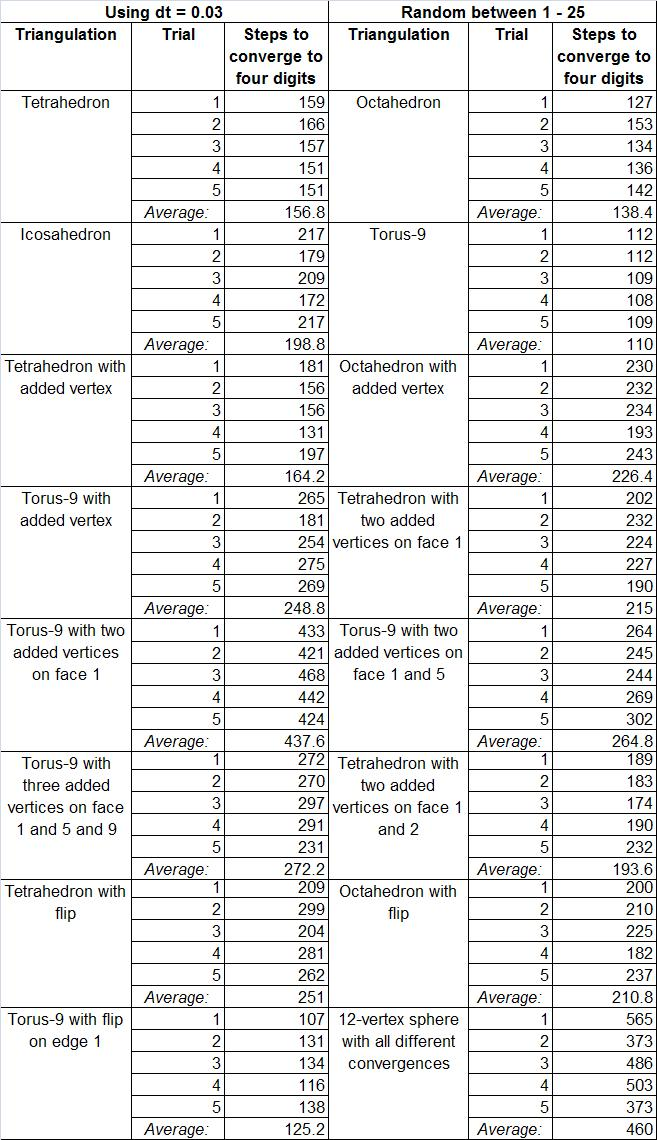
\includegraphics[scale = 0.7]{Pictures/ConvergenceTable.png}
\caption{Summary of convergence data for varying criteria}
\label{fig:conv}
\end{figure}

\noindent Beginning with the basic case, the tetrahedron took on average 156.8 steps to converge to four digits and remained fairly consistent through all five trials. Strangely, the octahedron converged faster on all five flows, averaging 138.4 steps. This was made all the stranger by the fact that the icosahedron averaged 198.8 steps. The torus revealed several things about convergences. First, the standard nine vertex torus averaged only 110 steps, suggesting that a torus converges faster than a sphere. When a vertex was added to the torus, it greatly decreased the convergence speed, to 248.8 steps. Compared to the Tetrahedron with an added vertex, 164.2, this was a very large jump. When another vertex was added to the same face as the first, the convergence speed dropped yet again, to an average of 437.6 steps. Yet when this vertex was added to a face not connected to the first, the convergence speed was almost steady at 264.8. And adding a third in the same style caused little increase.\newline

\noindent This seems to suggest that convergence speed is dependent on the number of unique vertices. By unique we mean the properties of the vertex (number of local vertices, the weight it converges to, etc.). When the vertices were added to separate faces, there remained only three unique vertices. Whereas, adding the two vertices to the same face created five unique vertices. This theory is further supported by a twelve vertex sphere designed so that all vertices are unique. The average convergence was 460 steps, more than twice as long as the icosahedron, which also is a twelve vertex sphere.\newline

\noindent As a final note, the deviation of the initial weights did not have a clear impact on the convergence speed. At some times, it would appear that initial weights with a higher deviation would converge faster, yet at other times it was lower deviation that seemed to lead to faster convergence.

\section{Spherical and hyperbolic Ricci flow}
\label{HypSphere}

So far we have focused exclusively on triangulations using Euclidean geometry. While this is useful for most cases, there are others where a different background space may be better suited. Two of these in particular are spherical and hyperbolic geometries. We will introduce the basics of each system to the reader as they may be unfamilar with these geometries. We will examine the adaptations of combinatorial Ricci flow for each case, test over various triangulations, and attempt to reach conclusions on our findings. 

\subsection{Spherical flow}
If you were to draw a large triangle on the surface of the earth, you would see that the line segments are no longer linear, but follow along an arc. In dealing with spherical geometry, we learn that many rules of planar geometry, some of them fundamental, do not apply. To begin, the sums of angles in a triangle do not add to $180^\circ$. The sum changes depending on the edge lengths. For computational reasons, we cannot (easily) have edges of unbounded length. While we can assume our circle packing metric still holds, we do have additional restrictions: 

\begin{itemize}
\item All triangles must be producable on a sphere of radius 1, the unit sphere. 
\item By default, we imply the geodesic of a spherical triangle, using the shortest distance on the surface between any two vertices. As a result, the sum of the weights of any triangle cannot exceed $\pi.$ In addition to contradicting the previous definition, such a situation can lead to undefined calculations of our angles, the equation of which is provided below.
\end{itemize}

\noindent We also have different formulas for numerous things in the spherical case. There are now two laws of cosines. One gives you an angle based on the edge lengths, like in Euclidean space, and the other gives you the side lengths based on the angles. For the first law of cosines, given a triangle with edge lengths $a, b$, and $c$, we have $\cos(\angle C) = \frac{\cos(c) - \cos(a)\cos(b)}{\sin(a)\sin(b)}$. Using Taylor polynomials to a couple of terms, we can see that this is analogous to the Euclidean version. With $\sin(x) \approx x$ and $\cos(x) \approx 1 - \frac{x^2}{2}$ for $x$ small, we get 
\begin{eqnarray*}
\cos(\angle C) &=& \frac{\cos(c) - \cos(a)\cos(b)}{\sin(a)\sin(b)} = \frac{(1 - \frac{c^2}{2}) - (1 - \frac{a^2}{2})(1 - \frac{b^2}{2})}{ab}\\
							&=& \frac{\frac{a^2}{2} + \frac{b^2}{2} - \frac{c^2}{2} + \frac{a^2b^2}{4}}{ab}\\
							&=& \frac{a^2 + b^2 - c^2}{2ab} + \frac{ab}{4} \approx \frac{a^2 + b^2 - c^2}{2ab} \mbox{ as } \frac{ab}{4} \approx 0 \mbox{ for } a,b \mbox{ small}
\end{eqnarray*}

\noindent More importantly, our equation for combintorial Ricci flow is altered slightly. The base equation, as given by \cite{chowluo}, is now 
\begin{equation}
\label{SRiccif}
\frac{dr_i}{dt} = -K_i\sin(r_i).
\end{equation}

\begin{figure}
\centering
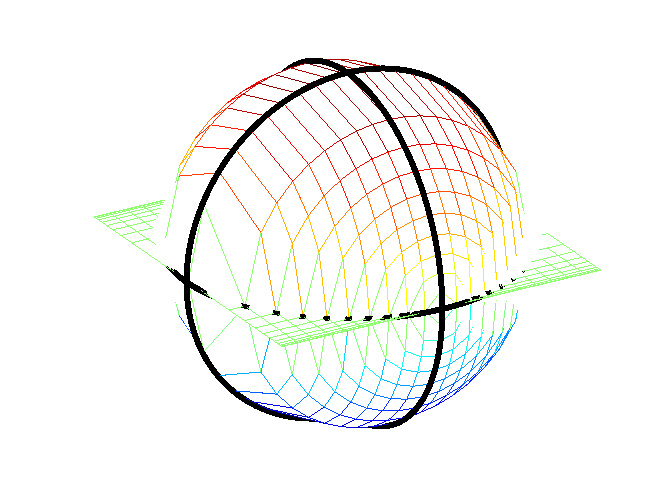
\includegraphics[scale = 0.6]{Pictures/octosph.png}
\label{OctoSph}
\caption{An illustration of a spherical octahedron through the X-Y plane. Each octet of the sphere surface, outlined in black, is the face of one triangle.} 
\end{figure}

\noindent Like in the Euclidean case, we see the possibility that all weights could continually decrease towards zero. However, scaling in the spherical case is not quite as easy as before: the angles are affected by the change in edge lengths. Plus, we also need to make sure that the weights remain within bounds.\newline

\noindent We tried a few techniques to derive an equation for normalized spherical flow. Some ideas were:

\begin{itemize}
\item $\displaystyle \frac{dr_i}{dt} = (\overline{K} - K_i)\sin(r_i)$ \newline
\noindent By maintaining the same construction as the normalized Euclidean Ricci flow, we hoped that replacing $r_i$ with $\sin(r_i)$ would work. However, in running even the simplest case of a tetrahdron, we found that the system was highly unstable. If more than one weight was initially different from the others, the program would fail. If the system was able to stabilize, we noted that the resultant surface area of the end product was $4\pi$, the same as a unit sphere. Another issue with this formula is that the value $\overline{K}$ is no longer constant. For a spherical construction of a surface $X$, we have 

$$\overline{K} = \frac{\sum{K_i}}{|V|} = \frac{2\pi\chi - \mbox{Surface Area of }X}{|V|}.$$

\noindent This is known as the Gauss-Bonnet theorem and is noted in Chow and Luo's paper \cite{chowluo}. Since the surface area went to $4\pi$, then the average curvature went to zero. While we liked the end result of our triangulation trials, the system failed far too often to be reliable. 

\item $\displaystyle \frac{dr_i}{dt} = (\hat{K} - K_i)r_i$ \newline
\noindent Following the criteria we used to obtain our normalized Euclidean flow, we began experimenting and used the cases $\tilde{r_i} = \alpha r_i$ and $\prod{\alpha \sin r_i} = C$ to obtain a result similar to our original. We defined $\hat{K}$ as the the dot product of the curvatures and the cosines of the weights, divided by the number of vertices, or 

$$\hat{K} = \frac{\sum{K_i \cos r_i}}{|V|}.$$

\noindent The major problem we encountered with this formula was that we had to use a sine approximation in its derivation, which is not valid for larger weights. As angles are not conserved with scaling in the spherical case, we realized this formula would not work. We also found that weights and curvatures displayed sinusoidal behavior, but were unable to converge to a finite value. As time went on, the weights became more unstable until the program reached failure, as seen in Fig.~\ref{kHat}.

\begin{figure}
\centering
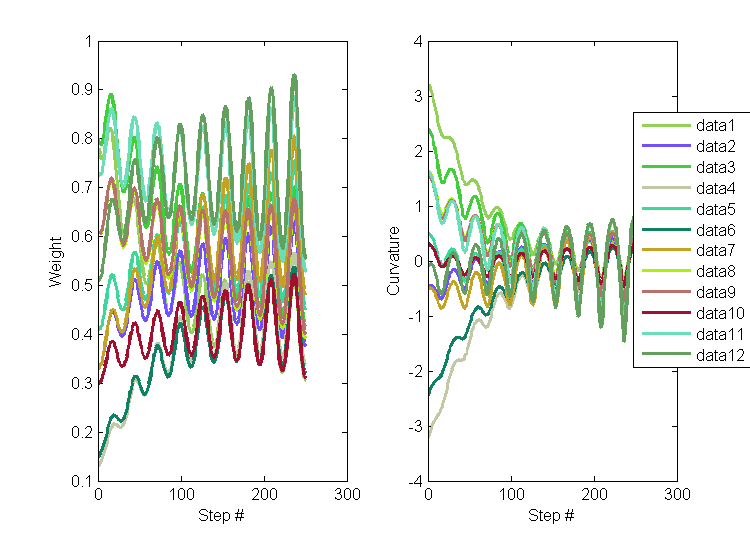
\includegraphics[scale = 0.65]{Pictures/kHatResult.png}
\caption{An example using our notion of $\hat{K}$. Weights and curvatures were unable to converge, and crashed the program shortly after.}
\label{kHat}
\end{figure}

\end{itemize}

\noindent In the end, we decided to try an equation that took the good aspects of our first trial while broadening its range of stability as we had hoped with the second one. We came up with the equation

\begin{equation}
\label{SRicciN}
\frac{dr_i}{dt} = \overline{K}r_i - K_i\sin(r_i).
\end{equation}

\noindent In examining its behavior with various triangulations, we found that this one works very well. We're not completely sure why, but it does. We would like to be able to mathematically determine the effectiveness of this equation. We find that spheres converge to zero curvature and weights first group together and then approach optimal weights. See Figure~\ref{SphGood}. In dealing with vertex transitive triangulations, ones in which each vertex has the same degree, we noted that sometimes all weights would converge to a specific value that was dependant on the number of vertices, and sometimes all the weights would be close to this number, but off by a small amount. In either case, the resulting surface area at the end turned out to be $4\pi$. For a vertex transitive genus 0 surface, we found that the preferred weight that each vertex approached or reached was equal to 

$$r_i = \frac{1}{2}\arccos(\frac{\cos(Z)}{1 - \cos(Z)}) \mbox{ where } Z = \frac{\pi(4 + F)}{3F}$$

\noindent and $F$ is the number of faces of the given triangulation. For example, with a tetrahedron, $F = 4, Z = \frac{2\pi}{3},$ and $r_i = \frac{1}{2}\arccos(-\frac{1}{3}) \approx 0.9553.$ The only downsides we found with this equation were that it was still possible for the system to fail if some weights got too large, and the computation time required to reach a stable equilibrium was lengthier than expected. Looking at Fig.~\ref{SphGood}, we see that with the $dt$ size given of $0.5$, it would take over 500 steps for the system to reach equilibrium, and this would be much longer with the $dt$ used in $\S\ref{InitialResults}$.  

\begin{figure}[ht]
\centering
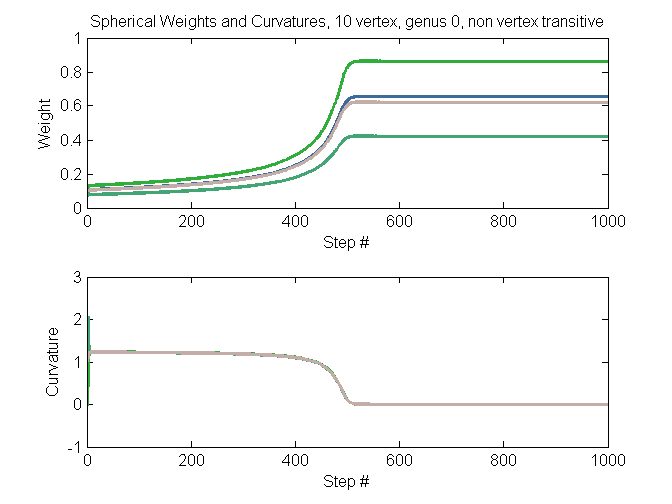
\includegraphics[scale = 0.8]{Pictures/SphG0V10.png}
\caption{An example of a solution using Eq.~(\ref{SRicciN}). Starting off with equal initial weights of 0.1, vertices merge into one of four groups as they approach uniform curvature relatively quickly. As curvature drops to zero, slowly at first but more forcefully as time passes, the weight groups separate from each other to obtain their final weight. In this trial, $dt = 0.50$ to show the complete process.}
\label{SphGood}  
\end{figure}

\subsection{Hyperbolic flow}

In hyperbolic geometry, we encounter a new background that has properties both similar and distinct from Euclidean and spherical systems. A common way to visualize the hyperbolic plane can be seen in Fig.~\ref{PD}. This representation is often called the Poincar\'{e} disk, named after the same Poincar\'{e} as in $\S$\ref{RBk}.\newline

\noindent There are several interesting properties with the hyperbolic plane. We now have that for a line $l$ and a point $P$ not on that line, there are an infinite number of lines throught $P$ that do not intersect $l$. In Euclidean geometry, such a line is unique. The shortest distance between two points is still a straight line, but illustratively can be found by following a curved path along a circle centered at infinity going through both points. A more thorough explanation of hyperbolic geometry can be found in most college geometry textbooks.\newline

\noindent In terms of the formulas, they remain relatively similar in format to the spherical equations, except there are two main substitutions. The cosine and sine functions are often replaced with their hyperbolic counterparts $cosh$ and $sinh$, defined as
\begin{eqnarray*}
\sinh(x) &=& \frac{e^x - e^{-x}}{2}\\
\cosh(x) &=& \frac{d\sinh(x)}{dt} = \frac{e^x + e^{-x}}{2}
\end{eqnarray*}

\noindent Most importantly, the equation for combinatorial Ricci flow is now
\begin{equation}
\label{HRiccif}
\frac{dr_i}{dt} = -K_i\sinh(r_i)
\end{equation}
\noindent 

\noindent Like in the case of spherical flow, the average and total curvatures need not remain constant. The average curvature is now
$$\overline{K} = \frac{\sum{K_i}}{|V|} = \frac{2\pi\chi + \mbox{Surface Area of }X}{|V|}.$$

\begin{figure}
\centering
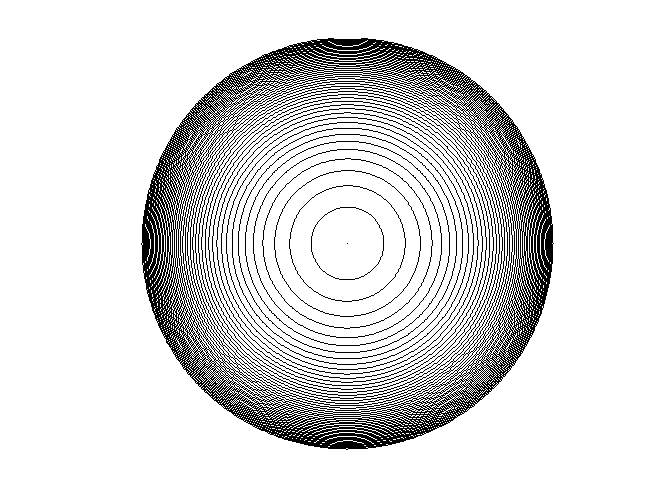
\includegraphics[scale = 0.5]{Pictures/pDisk.png}
\caption{An illustration of the hyperbolic plane using the Poincar\'{e} disk. All concentric circles are evenly spaced apart in a Euclidean background, but the outer edge of the disk approaches infinity, so the circles appear closer together. A similar way to think of it is to imagine looking at the contour graph of $z = x^2 + y^2$ from the point (0,0,-1).}
\label{PD}
\end{figure}

\noindent After running the hyperbolic Ricci flow on a few samples, we noted that the weights did not always go to zero, as was the case with the previous unnormalized systems. So in some cases, it almost seems as if this equation is already normalized. Curvatures would converge to zero, and optimum, nonzero weights are achieved in a relatively short time. Other times it behaved like both Euclidean and spherical. 

\subsection{Comparison of Systems}

When we began looking into these background geometries, we thought that it would be a good idea to run uniform tests on all three systems. We could observe whether or not each triangulation converges in the same fashion, or if it matters which geometry we choose. If we do discover that all systems behave the same way, we would then like to focus on one geometry, most likely Euclidean. However, since our equation for normalized spherical Ricci flow is not wholly confirmed as the best method, and as the hyperbolic flow may or may not already be normalized, we can not make any strong conclusions on the normalized flows. We did decide, however, to take a look at the behaviors on various manifolds by using the non-normalized equations, (\ref{Riccif}), (\ref{SRiccif}), and (\ref{HRiccif}). We will look at three triangulations, each of a different genus, without performing any morphs, and compare results between each system. \newline

\noindent In terms of programming these new flows, we were able to adapt our calcFlow program into two new programs, sphericalCalcFlow and hyperbolicCalcFlow, to easily distinguish which background we were using. This way we could run the systems one at a time, or all at once and observe differences in their behaviors in cases with the same initial conditions. \newline

\noindent \textit{Example:} 12 vertex sphere, vertex transitive of degree 5\newline

\noindent Euclidean- As expected, we obtain a surface where all the vertices attain the same curvature of $\frac{\pi}{3}$ after multiple trials of uniform and randomized weights. The weights group together somewhat as in the normalized spherical case, and then continue decreasing towards zero.\newline

\noindent Spherical- We found that the system was truly stable with nonzero final weights if and only if all initial weights were set exactly to its preferred weight, which is $\approx$ 0.55357 based on the fact that this triangulation has 20 faces. If the initial curvature was below zero, the weights would increase rapidly until the program crashed. If the initial curvature was positive, the vertices would approach the same curvature as in the Euclidean case. In doing so, the weights would drop to zero.\newline

\noindent Hyperbolic- We found that the vertices react in a similar manner to the Euclidean case. They approach the same curvature of $\frac{\pi}{3}$ and drop towards zero weights at the same rate.\newline 

\noindent \textit{Example:} 9 vertex, one-holed torus\newline

\noindent Euclidean- Since we know that $\chi = 0$ for a one-holed torus, we also know that $\overline{K} = 0$ and so each vertex obtains zero curvature. The weights do not drop to zero, but converge to positive values reflective of their degree. \newline

\noindent Spherical- We found this system to be very unstable with the torus. If the initial weights were too large, we found that the total curvature would be well below zero, and the weights would continually increase until sphericalCalcFlow crashed. While we hoped that reducing the initial weights would bring stability to the system, we ended up with the same result.

\noindent Hyperbolic- While the total curvature of the system goes to zero, the weights also approach zero but maintain roughly the same proportion as the final Euclidean weights. Another thing we noted was the time required for the weights and curvatures to go to zero. This system was extremely slow and took much longer than either the Euclidean or spherical trials. \newline

\noindent \textit{Example:} 11 vertex, two-holed torus\newline

\noindent Euclidean- As in previous cases, the vertices converge to a uniform curvature. However, as this value was negative (given $\chi = -2$) we saw the weights increase without bound. As there is no limit to the weights in the Euclidean case, calcFlow had no troubles calculating each iteration, but having unbounded weights is still an undesired result. \newline

\noindent Spherical- Regardless of the initial weights, we found that the total curvature of the system would continually decrease, and as such the weights of each vertex would increase until sphericalCalcFlow crashed. \newline

\noindent Hyperbolic- Here we found that hyperbolic geometry was very effective. In a very short time, we saw the vertices reach zero curvature, and the weights converge to nonzero values. This is how we got our notion that the hyperbolic Ricci flow was already normalized. This also coincides with the suggestion in \cite{chowluo}; when working with a negative euler characteristic manifold, one should use hyperbolic geometry.\newline

\noindent To conlude, we generalize that certain flows work best for triangulations whose total curvature goes to zero in that particular system. Euclidean is best for systems of genus 1, or one-holed tori. Spherical combinatorial Ricci flow is said to work best on manifolds of genus 0, or anything topologically equivalent to a sphere. This is because we have a positive $\chi$ value, so for total curvature to go to 0, the total surface area must go to $4\pi$. Spherical was the only system that could have produced a nontrivial solution in our first example. Hyperbolic Ricci flow is best suited for triangulations with a genus of 2 or more. We can see that these systems will be able to reach zero total curvature with a large enough surface area. 
\section{Future work}
\label{Future}

\subsection{Linking Delaunay to Ricci flow}
Delaunay surfaces and combinatorial Ricci flows can seem to be very separate concepts, and in many ways with our program structure, they are. Yet there is the possiblity of combining both of them to explore other mathematical inquiries. For instance, how does the idea of Delaunay triangles interact with triangulations on a manifold. We know that a circle packed triangulation is weighted Delaunay, but what if the triangulation is not circle packed (see below)? Will the Ricci flow lead to a weighted Delaunay triangulation?

\subsection{Circle packing expansions}
\label{circExt}
Circle packing is a very special way to characterize our side lengths. If we relax this criteria and let the circles overlap, we can introduce a second weight $\Phi$ that is representative of the angle of their intersection. See Figure \ref{fig:intcirc}. We can then evaluate our side lengths as $$l_{ij} = \sqrt{r_i^2 + r_j^2 + 2r_ir_j\cos(\Phi(e_{ij}))}$$ With this more general interpretation, we can examine questions asked by Chow and Luo in \cite{chowluo}.

\begin{figure}
\begin{center}
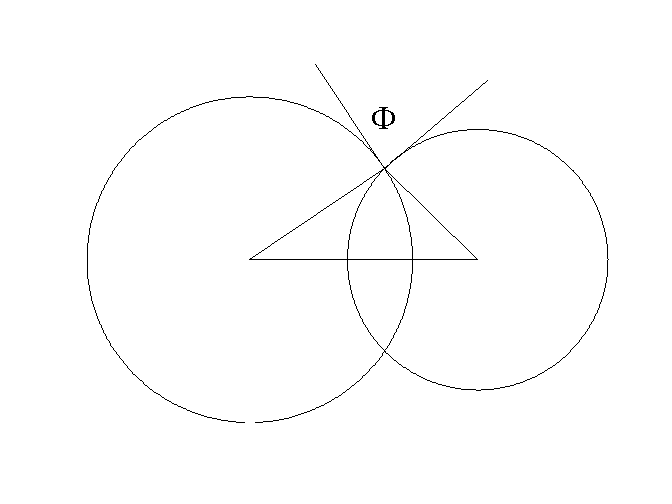
\includegraphics[scale = 0.6]{Pictures/intcirc2.png}
\end{center}
\caption{An example of relaxing circle packing and introducing $\Phi.$}
\label{fig:intcirc}
\end{figure}

\subsection{3-Dimensional triangulations}
Triangulations exist outside of two dimensions and one future goal is to perform flows in a three dimensional setting. The flow in this case is known as Yamabe flow, discussed in \cite{DrG}. While Yamabe flow is similar to Ricci flow, its value of $K_i$ is determined quite differently, involving not only the angles of the faces, but also the cone angles associated with tetrahedron vertices. The structure is in place from this project to accomplish this goal. To help the understanding of both the two and three dimensional triangulations, we would like to create a way to visualize them and explore the surfaces locally.\newline

\section{Conclusion}

We had a lot of goals for this project. For one, we are the first group to work with Dr. David Glickenstein and he has his own long-term goals. As the initial builders for these goals, we feel that we have laid a good foundation that can be easily built upon by future undergraduate students. We are excited to see where Dr. Glickenstein's project is headed and we hope to remain a part of it in the months and years to come. Another goal was to properly implement Ricci flow for 2-dimensional manifolds. While there are a number of extensions that still need to be implemented, we are pleased that the flow is functional and providing useful data. Our jump to weighted Delaunay triangulations enabled us to make our code more adaptable, as well as be able to generate our own systems with desired properties. We also feel we have learned an enormous amount over the course of only a few weeks. At the beginning, we all had varying familiarities with college geometry; some of us had not had a course in geometry since high school. Lastly, the experience from writing a research report will undoubtedly help us in our future endeavors. We would like to thank Dr. David Glickenstein for having us on this project, Dr. Robert Indik and the University of Arizona Math Department for their help and support, and the National Science Foundation VIGRE $\#$0602173.

\newpage
\bibliography{Test1}  
\bibliographystyle{plain}

\newpage
\section{Appendix}

\subsection{Derivation of Eq.~(\ref{proof1})}
\maketitle
	
	We used the criteria $$f(\tilde{r_1},\tilde{r_2},\ldots,\tilde{r_n}) = \prod{\tilde{r_i}} = \prod{\alpha r_i} = \alpha^n\prod{r_i}= C$$ to constrain the values of radii. We take the derivative of $f$ with respect to $t$ and obtain
	\begin{eqnarray*}
	\frac{df}{dt} & = & n\alpha^{n-1}\frac{d\alpha}{dt}r_1r_2\ldots r_n + \alpha^n\frac{dr_1}{dt}r_2r_3\ldots r_n\\
								& + & \alpha^nr_1\frac{dr_2}{dt}r_3r_4\ldots r_n + \ldots + \alpha^nr_1r_2\ldots r_{n-1}\frac{dr_n}{dt}.
	\end{eqnarray*}
	But since $\displaystyle \frac{dr_i}{dt} = -K_ir_i$ from Eq.~(\ref{Riccif}) we obtain
	\begin{eqnarray*}
	\frac{df}{dt} & = & \frac{n\alpha^{n}}{\alpha}\frac{d\alpha}{dt}r_1r_2\ldots r_n - K_1\alpha^nr_1r_2r_3\ldots r_n\\
								& - & K_2\alpha^nr_1r_2r_3r_4\ldots r_n - \ldots - K_n\alpha^nr_1r_2\ldots r_{n-1}r_n
	\end{eqnarray*}
	from which we can group terms and obtain
	\begin{eqnarray*}
	\frac{df}{dt} & = & (\alpha^nr_1r_2\ldots r_n)(\frac{n}{\alpha}\frac{d\alpha}{dt} - K_1 - K_2 - \ldots - K_n)\\
								& = & C(\frac{n}{\alpha}\frac{d\alpha}{dt} - K_1 - K_2 - \ldots - K_n).
	\end{eqnarray*}
	If we assume the product is a constant, we have $\displaystyle \frac{df}{dt} = 0.$ Thus we have $$\frac{n}{\alpha}\frac{d\alpha}{dt} - K_1 - K_2 - \ldots - K_n = 0.$$
	Rearranging we have
$$\frac{1}{\alpha}\frac{d\alpha}{dt} = \frac{d(\log \alpha)}{dt} = \frac{K_1 + K_2 + \ldots + K_n}{n} = \overline{K}$$
	which we refer to as Eq.~(\ref{proof1})
  
  \subsection{Remarks on Runge-Kutta method for solving Eq.~(\ref{Riccin})}
	\maketitle

The method used by Moreau in \cite{JPM} to solve a differential equation involves using a Runge-Kutta method. Prior to adapting the code from Moreau's website, we reached the conclusion that a Runge-Kutta format would be most beneficial for this type of differential equation problem. Even though it is more computationally complex than the simpler Euler's method, it makes up in its ability to converge and in its accuracy. According to $\cite{DiffEq}$ the error associated with using Runge-Kutta is on the order of $h^4$, whereas with a standard Euler approximation the error is simply of order $h$, with $h = dt$ being our step incremental.\newline

\noindent Based on our evaluations of radii and curvatures over time, it appears to converge exponentially for each vertex. However, as mentioned previously, performing flips on a triangulation may create unusual behavior.

\subsection{Data Plots}
\label{dataplots}

\begin{figure}[h]
\begin{center}
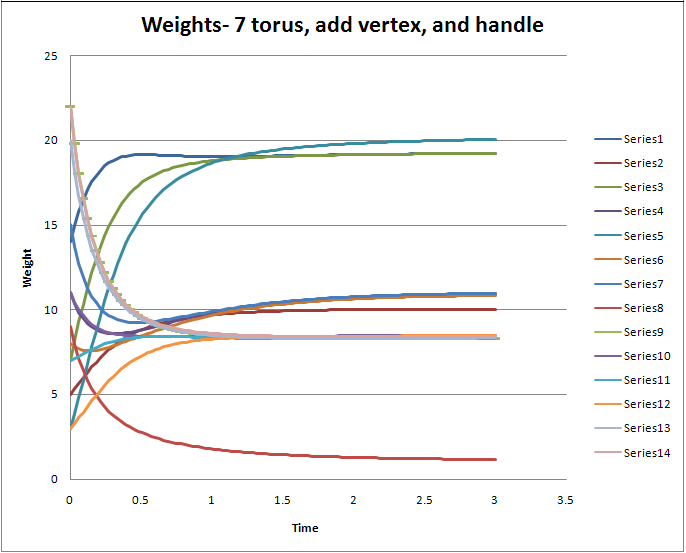
\includegraphics[scale = 0.65]{Pictures/torus7addvaddhweights2.png}
\caption{An example of how morphs can change the asymptotic behavior of vertices. In this case we saw the weights of some vertices change concavity.}
\label{fig:t7vh}
\end{center}
\end{figure}

\begin{figure}
\begin{center}
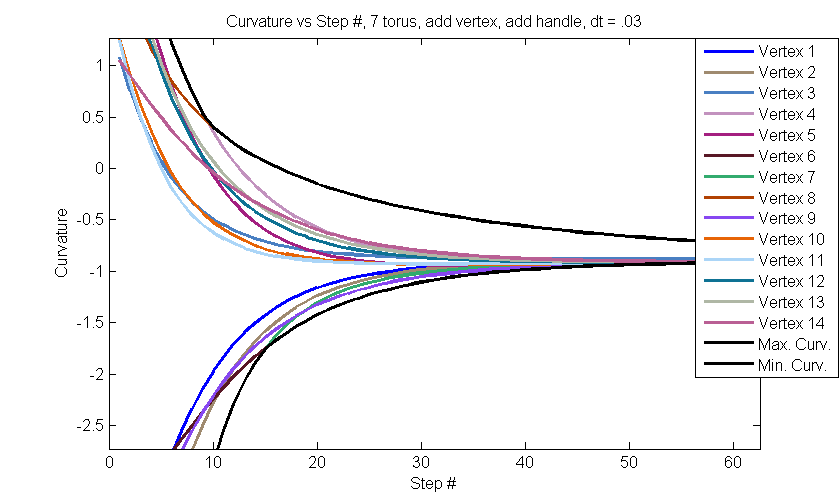
\includegraphics[scale = 0.8]{Pictures/curvcurves.png}
\caption{An example of curvatures over time. While they do converge to the same curvature, the vertex with the maximum or minimum curvature may change. This is a separate trial than that producing Fig.~\ref{fig:t7vh}}
\end{center}
\end{figure}

\begin{figure}
\begin{center}
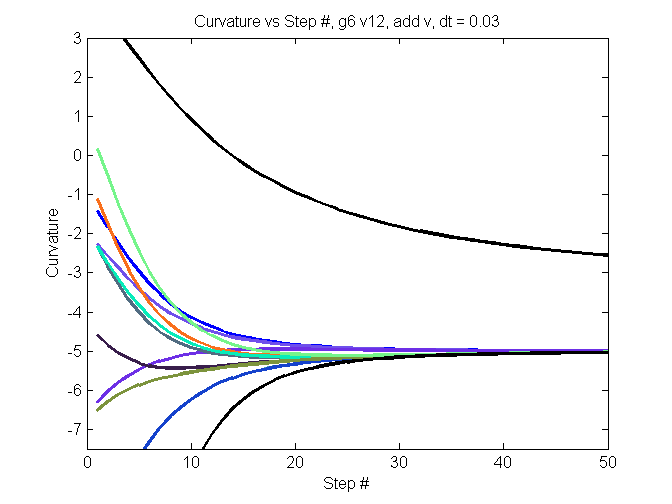
\includegraphics[scale = 0.7]{Pictures/Curvg6v12addv.png}
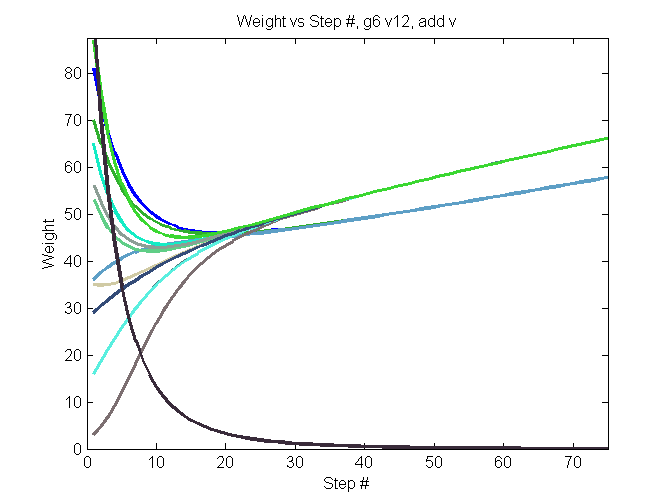
\includegraphics[scale = 0.7]{Pictures/Weightg6v12addv.png}
\caption{An example of adding a vertex to a genus 6 surface. One of the curvatures in unable to drop below $-\pi$, and as a result, its weight is pushed to almost zero. Other vertices group together to compensate for this behavior.}
\end{center}
\end{figure}

%\newpage
\subsection{Code Examples}

\noindent Code from the program can be found here: http://code.google.com/p/geocam. \newline

\begin{figure}
\begin{center}
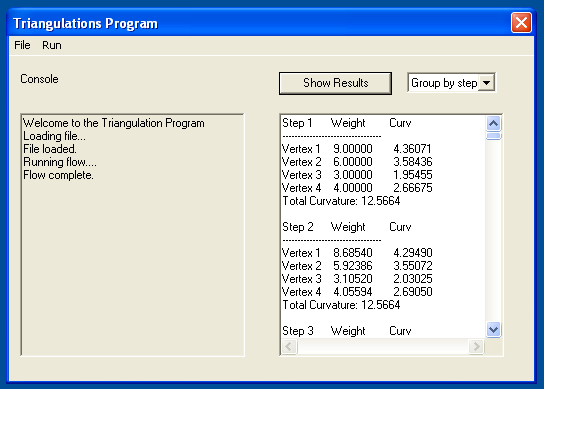
\includegraphics[scale = 0.65]{Pictures/GUIpic.png}
\caption{A snapshot of the user interface written to run both Ricci flows and Delaunay flip algorithms. Results of a flow are written in a text field on the right.}
\end{center}
\end{figure}

\noindent The \textit{clacFlow} method calculates the combinatorial Ricci flow of the current Triangulation using the Runge-Kutta method. Results from the steps are written into vectors of doubles provided. The parameters are:\newline

\begin{itemize}
\item\textbf{vector$<$double$>$* weights-} A vector of doubles to append the results of weights, grouped by step, with a total size of numSteps * numVertices.
\item\textbf{vector$<$double$>$* curvatures-} A vector of doubles to append the results of curvatures, grouped by step, with a total size of numSteps * numVertices. The time step size. Initial and ending times not needed since diff. equations are independent of time.
\item\textbf{double* initWeights-} Array of initial weights of the Vertices in order.
\item\textbf{int numSteps-} The number of steps to take. (dt = (tf - ti)/numSteps)
\item\textbf{bool adjF-} Boolean of whether or not to use adjusted differential equation. True to use adjusted.
\end{itemize}

\noindent The information placed in the vectors are the weights and curvatures for each Vertex at each step point. The data is grouped by steps, so the first vertex of the first step is the beginning element. After n doubles are placed, for an n-vertex triangulation, the first vertex of the next step follows. If the vectors passed in are not empty, the data is added to the end of the vector and the original information is not cleared.

\label{calcFlowCode}
\begin{verbatim}
void calcFlow(vector<double>* weights, vector<double>* curvatures, double dt, 
              double* initWeights, int numSteps, bool adjF)  
{
  int p = Triangulation::vertexTable.size(); // The number of vertices or 
                                             // number of variables in system.
                                         
  double ta[p],tb[p],tc[p],td[p],z[p]; // Temporary arrays to hold data for 
                                      // the intermediate steps in.
  int    i,k; // ints used for "for loops". i is the step number,
              // k is the kth vertex for the arrays.
  map<int, Vertex>::iterator vit; // Iterator to traverse through the vertices.
  // Beginning and Ending pointers. (Used for "for" loops)
  map<int, Vertex>::iterator vBegin = Triangulation::vertexTable.begin();
  map<int, Vertex>::iterator vEnd = Triangulation::vertexTable.end();
  
  double net = 0; // Net and prev hold the current and previous
  double prev;    //  net curvatures, repsectively.
   for (k=0; k<p; k++) {
    z[k]=initWeights[k]; // z[k] holds the current weights.
   }
   for (i=1; i<numSteps+1; i++)
   {  // This is the main loop through each step.
    prev = net; // Set prev to net.
    net = 0;    // Reset net.
    
       for (k=0, vit = vBegin; k<p && vit != vEnd; k++, vit++)  
       {
           // Set the weights of the Triangulation.
           vit->second.setWeight(z[k]);
       }
       if(i == 1) // If first time through, use static method to 
       {           // calculate total cuvature.
            prev = Triangulation::netCurvature();
       }
       for (k=0, vit = vBegin; k<p && vit != vEnd; k++, vit++) 
       {  // First "for loop"in whole step calculates everything manually.
           (*weights).push_back( z[k]); // Adds the data to the vector.
           double curv = curvature(vit->second);
           if(curv < 0.00005 && curv > -0.00005) 
           {  // Adjusted for small numbers. We want it to print nicely.
             (*curvatures).push_back(0.); // Adds the data to the vector.
           }
           else {
               (*curvatures).push_back(curv);
           }
           net += curv; // Calculating the net curvature.
           // Calculates the differential equation, either normalized or
           // standard.
           if(adjF) ta[k]= dt * ((-1) * curv 
                           * vit->second.getWeight() +
                           prev /  p
                           * vit->second.getWeight());
           else     ta[k] = dt * (-1) * curv 
                           * vit->second.getWeight();
           
       }
       for (k=0, vit = vBegin; k<p && vit != vEnd; k++, vit++)  
       { // Set the new weights to our triangulation.
           vit->second.setWeight(z[k]+ta[k]/2);
       }
       for (k=0, vit = vBegin; k<p && vit != vEnd; k++, vit++)  
       {
            // Again calculates the differential equation, but we
            // still need the data in ta[] so we use tb[] now.
            if(adjF) tb[k]=dt*adjDiffEQ(vit->first, net);
            else     tb[k]=dt*stdDiffEQ(vit->first);
       }
       for (k=0, vit = vBegin; k<p && vit != vEnd; k++, vit++)  
       { // Set the new weights.
           vit->second.setWeight(z[k]+tb[k]/2);
       }
       for (k=0, vit = vBegin; k<p && vit != vEnd; k++, vit++)  
       {
            if(adjF) tc[k]=dt*adjDiffEQ(vit->first, net);
            else     tc[k]=dt*stdDiffEQ(vit->first);
       }
       for (k=0, vit = vBegin; k<p && vit != vEnd; k++, vit++)  
       { // Set the new weights.
           vit->second.setWeight(z[k]+tc[k]);
       }
       for (k=0, vit = vBegin; k<p && vit != vEnd; k++, vit++)  
       {
            if(adjF) td[k]=dt*adjDiffEQ(vit->first, net);
            else     td[k]=dt*stdDiffEQ(vit->first);
       }
       for (k=0; k<p; k++) // Adjust z[k] according to algorithm.
       {
         z[k]=z[k]+(ta[k]+2*tb[k]+2*tc[k]+td[k])/6;
         
       }
   }
}
\end{verbatim}

\section*{About the authors}

Alex Henniges is a junior double majoring in Math and Computer Science. Thomas Williams is a senior in Comprehensive Mathematics with a minor in Computer Science and a background in Math Education. Mitch Wilson is a senior double majoring in Applied Math and Mechanical Engineering.\newline

\noindent Contact information:
\begin{itemize}
\item Dr. David Glickenstein- glickenstein@math.arizona.edu
\item Alex Henniges- henniges@email.arizona.edu
\item Thomas Williams-
\item Mitch Wilson- mjw@email.arizona.edu
\end{itemize}
\noindent Project website: http://code.google.com/p/geocam

\end{document}